\documentclass{article}
\usepackage{graphicx}  % To include the visualization image
\usepackage{hyperref}  % For hyperlinks
\usepackage{geometry}  % For adjusting margins
\geometry{a4paper, margin=1in}

\title{FIT3179 Week 9 Homework Report}
\author{Jarel Eloysius Gomes, 33600414}
\date{\today}

\begin{document}

\maketitle

\section*{Introduction}
This report presents a proportional symbol map visualizing the public transport ridership in Malaysia. The map highlights the daily ridership across various locations in Malaysia using circles with varying sizes based on ridership values. The map was generated using Vega-Lite and published on GitHub Pages. Data was cleaned and sourced from public ridership datasets, focusing on key transport hubs across Malaysia.

\section*{Data Description}
The data used for this visualization was a cleaned CSV dataset containing information on public transport ridership across different regions in Malaysia. The key columns of the dataset are:
\begin{itemize}
    \item \textbf{Location:} Name of the public transport hub or city.
    \item \textbf{Latitude:} Latitude coordinates for the location.
    \item \textbf{Longitude:} Longitude coordinates for the location.
    \item \textbf{Ridership:} The daily ridership numbers, which are quantitative values.
\end{itemize}

The dataset was pre-processed to exclude any entries where the ridership value was null or zero, ensuring that only meaningful and valid data points were included in the map. This resulted in an accurate and informative visualization.

\section*{Data Transformation}
No major transformations were applied to the dataset beyond filtering out invalid entries (null or zero ridership). The dataset did not require normalization by area or population, as the visualization aimed to display point-specific data (i.e., transport hubs) rather than regional comparisons.

\section*{Visualization Design}
The proportional symbol map uses an \textbf{equirectangular projection}, centered on Malaysia. Circles represent public transport hubs, with their sizes corresponding to daily ridership values. The map includes three layers:
\begin{itemize}
    \item \textbf{Base Map:} Malaysia’s geographic boundaries are represented using a TopoJSON file.
    \item \textbf{Proportional Symbols:} Circles vary in size according to ridership data. Larger circles indicate higher ridership, making it easy to compare transport hubs.
    \item \textbf{Graticule:} A grid of latitude and longitude lines provides context for the geographic layout.
\end{itemize}

The circle sizes are scaled between 0 and 100,000, corresponding to ridership values. The graticule adds geographic orientation, making the map easy to interpret.

\begin{figure}[h!]
    \centering
    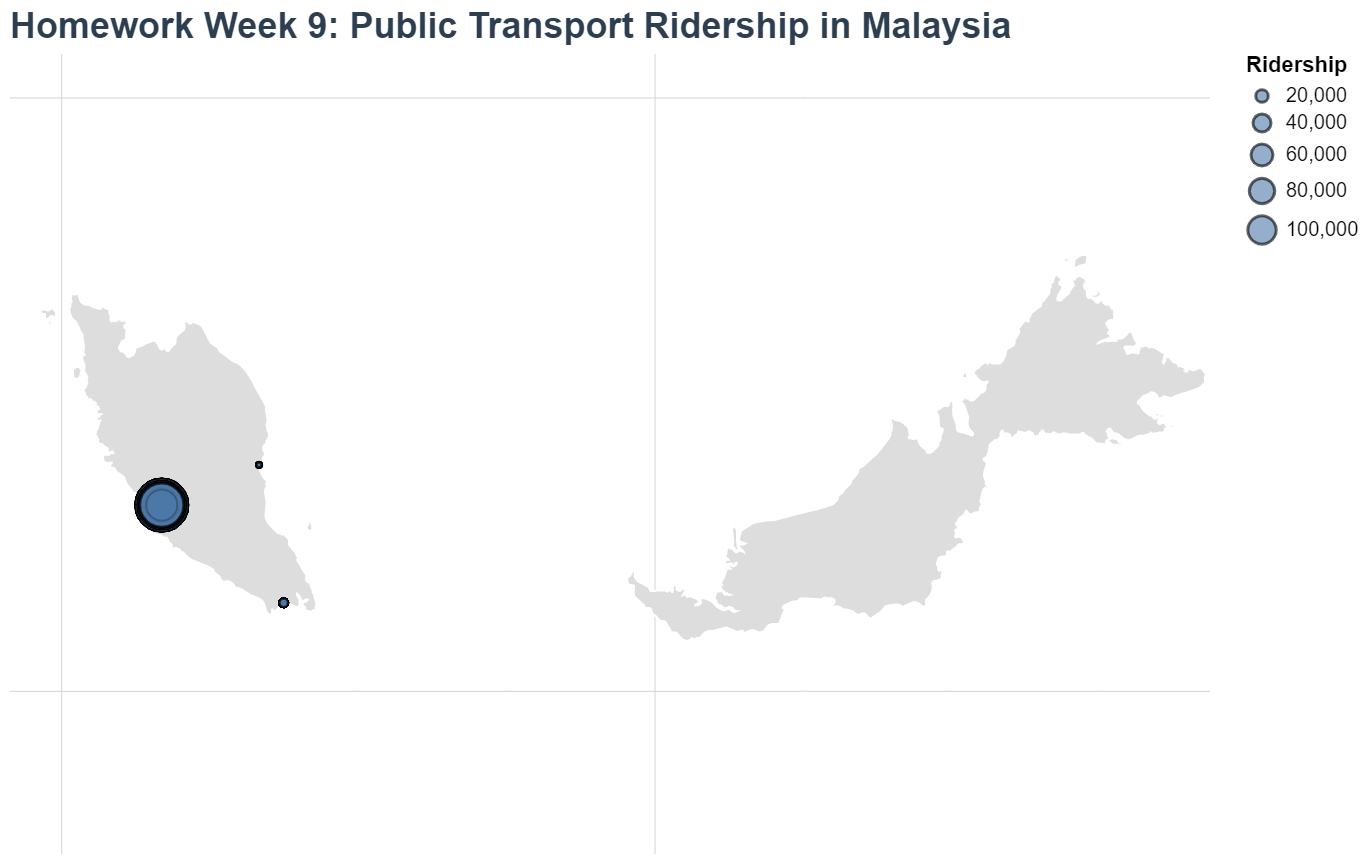
\includegraphics[width=\textwidth]{week9hwvisualization.png}
    \caption{Proportional symbol map showing public transport ridership in Malaysia.}
\end{figure}

\section*{Map Justification}
A proportional symbol map was chosen because it allows for the clear representation of ridership volume at individual transport hubs. This type of map is ideal when visualizing point-based data (i.e., transport stations) rather than regions, making it superior to other map types in this context:
\begin{itemize}
    \item A \textbf{choropleth map} would not have been appropriate since ridership data is not region-based but rather specific to transport hubs.
    \item A \textbf{dot map} could have been an option, but it would fail to convey the magnitude of ridership differences as effectively as proportional symbols.
\end{itemize}

The chosen map provides an intuitive comparison of ridership volumes by varying the size of circles, with the exact values displayed in tooltips for additional detail.

\section*{Conclusion}
The proportional symbol map effectively visualizes public transport ridership across different locations in Malaysia. By using circles to represent ridership levels at various transport hubs, the map provides an easy-to-understand comparison of ridership volumes. This design, combined with the graticule for geographic orientation, presents the data clearly and accurately.

\section*{Links}
You can view the interactive version of this map on \href{https://github.com/jarelgomes1/week9fit3179HW}{GitHub Pages}.

\end{document}
